\begin{ex}
(Ufes) Num aparelho eletrônico, as dez teclas numeradas estão dispostas em fileiras horizontais, conforme indica a figura:
 \begin{center}
     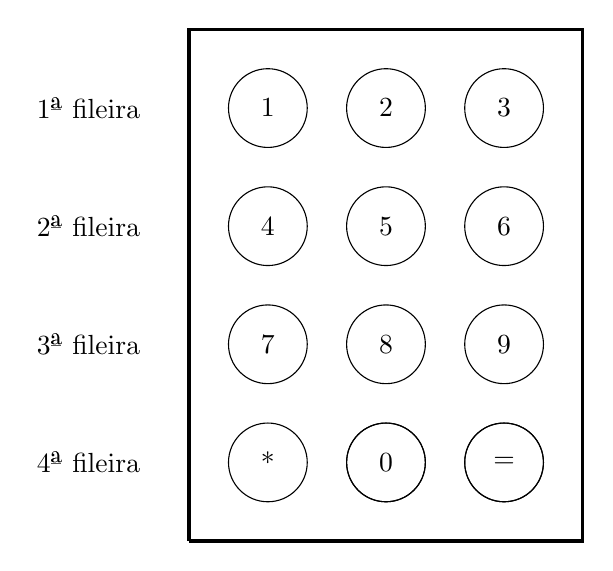
\begin{tikzpicture}
      \draw[very thick] (0,0)--(5,0)--(5,6.5)--(0,6.5)--(0,0); 
      \draw (1,1) circle [radius = .5];\draw  (2.5,1) circle [radius = .5];
      \draw (4,1) circle [radius = .5]; \draw (1,2.5) circle [radius = .5];\draw (1,4) circle [radius = .5]; \draw (1,5.5) circle [radius = .5]; \draw (2.5,1) circle [radius = .5];\draw (2.5,2.5) circle [radius = .5];\draw (2.5,4) circle [radius = .5];\draw (2.5,5.5) circle [radius = .5]; \draw (4,1) circle [radius = .5];\draw (4,2.5) circle [radius = .5];\draw (4,4) circle [radius = .5]; \draw (4,5.5) circle [radius = .5];\node at (1,1) {*}; \node at (2.5,1) {0};
      \node at (4,1) {=}; \node at (1,2.5) {7}; \node at (2.5,2.5) {8};
       \node at (4,2.5) {9}; \node at (1,4) {4}; \node at (2.5,4) {5};
       \node at (4,4) {6}; \node at (1,5.5) {1}; \node at (2.5,5.5) {2};
       \node at (4,5.5) {3};
       \node at (-.5,1) [left] {4ª fileira};\node at (-.5,2.5) [left] {3ª fileira}; \node at (-.5,4) [left] {2ª fileira}; \node at (-.5,5.5) [left] {1ª fileira};
     \end{tikzpicture}
 \end{center}
Seja N a quantidade de números de telefone com 8 dígitos, que começam pelo dígito 3 e terminam pelo dígito zero, e, além disso, o 2º e o 3º dígitos são da primeira fileira do teclado, o 4º e o 5º são da segunda fileira, e o 6º e o 7º são da terceira fileira. O valor de N é:
   \begin{enumerate}[(a)]
   \item 27
   \item 216
   \item 512
   \item 729
   \item 1331
   \end{enumerate}
     \begin{sol}
     resposta: d \\
     $\frac{3}{1}\frac{\phantom{A}}{3}\frac{\phantom{A}}{3}\frac{\phantom{A}}{3}\frac{\phantom{A}}{3}\frac{\phantom{A}}{3}\frac{\phantom{A}}{3}\frac{0}{1}=3^6 \Longrightarrow N=729$
     \end{sol}
\end{ex}